\setcounter{chapter}{2}

\chapter{函数极限与连续}

\section{函数极限的概念与性质}

\subsection{函数极限的概念}

{\bf 函数极限的六种不同趋势}

\begin{itemize}
  \setlength{\itemindent}{1cm}
  \item 趋于无穷
  $$x\to\infty,\quad x\to+\infty,\quad x\to-\infty$$
  \item 趋于有限值
  $$x\to x_0,\quad x\to x_0^+,\quad x\to x_0^-$$
\end{itemize}

{\bf 思考:} $\limn f(n)=A\Leftrightarrow\limx{+\infty}f(x)=A$?($\times$)

\subsubsection{趋于无穷时的函数极限}

{\bf 定义3.1.1}
\begin{enumerate}[(1)]
  \setlength{\itemindent}{1cm}
  \item $\limx{+\infty}f(x)=A\Leftrightarrow\forall \e>0,\exists X,\forall
  x>X,|f(x)-A|<\e$
  \item $\limx{-\infty}f(x)=A\Leftrightarrow\forall \e>0,\exists X,\forall
  x<X,|f(x)-A|<\e$
  \item $\limx{+\infty}f(x)=A\Leftrightarrow\forall \e>0,\exists X,\forall
  |x|>X,|f(x)-A|<\e$
\end{enumerate}

{\bf 注:}和$\limn a_n=a$的定义做类比,理解(1),然后推广到(2),(3)。特别是有关的性质,如
\begin{itemize}
  \setlength{\itemindent}{1cm}
  \item $A$必须是确定值
  \item $\e$可以任意小
  \item $X$要充分大(或小)
  \item 不等式右端可以乘以某个常数$C$
\end{itemize}

{\bf 定义3.1.2}
\begin{enumerate}[(1)]
  \setlength{\itemindent}{1cm}
  \item $\limx{x_0}f(x)=A\Leftrightarrow\forall \e>0,\exists\delta>0,\forall
  x\in U_0(x_0,\delta),|f(x)-A|<\e$
  \item $\limx{x_0^+}f(x)=A\Leftrightarrow\forall \e>0,\exists\delta>0,\forall
  x\in(x_0,x_0+\delta),|f(x)-A|<\e$
  \item $\limx{x_0^-}f(x)=A\Leftrightarrow\forall \e>0,\exists\delta>0,\forall
  x\in(x_0-\delta,x_0),|f(x)-A|<\e$
\end{enumerate}

{\bf 例}(习题3.1-1)根据图形判断极限的存在性
\begin{center}
	\resizebox{!}{4cm}{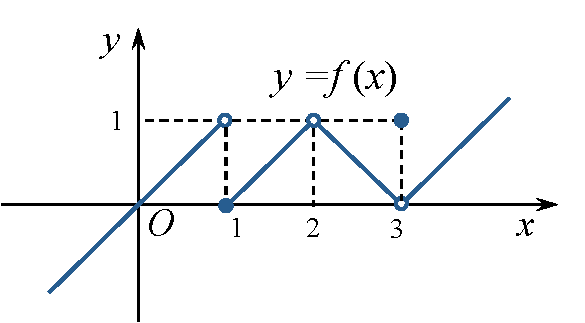
\includegraphics{./images/ch3/limxf.pdf}}
\end{center}
\begin{enumerate}[(1)]
  \setlength{\itemindent}{1cm}
  \item $\limx{1}f(x)$\underline{不存在}
  \item $\limx{2}f(x)$\underline{$=1$}
  \item $\limx{1}f(x)$\underline{$=0$}
\end{enumerate}

{\bf 思考:}
\begin{itemize}
  \setlength{\itemindent}{1cm}
  \item 为什么在定义中要求$0<|x-x_0|<\delta$,而不是$|x-x_0|<\delta$?
  {\it (因为极限表示一种趋势,与函数在该点处的取值无关)}
  \item $f(x_0+0),f(x_0-0)$与$f(x_0)$是何关系?
  {\it(前两者分别表示左右极限,最后一个是函数值,三者相互无关)}
\end{itemize}

{\bf 例:}证明
\begin{enumerate}[(1)]
  \setlength{\itemindent}{1cm}
  \item $\limx{1}\df1x=1$
  \item $\limx{x_0}\sin x=\sin x_0$
\end{enumerate}

\begin{shaded}
	{\bf 【函数极限的反面说法】}
	
	\begin{itemize}
	  \item 当$x\to x_0$时$f(x)$不以$A$为极限 
	    $$\exists\e_0>0,\forall\delta>0, \exists x^*\in
	    U_0(x_0,\delta),|f(x^*)-A|\geq\e_0$$ 
	  \item 当$x\to x_0$时$f(x)$无极限
		$$\forall A\in\mathbb{R},\exists\e_0>0,\forall\delta>0, \exists x^*\in
	    U_0(x_0,\delta),|f(x^*)-A|\geq\e_0$$ 
	\end{itemize}
	
	{\bf 例:}证明:Dirichlet函数在任意点处无极限。
\end{shaded}

{\bf 课堂思考:}
\begin{enumerate}[(1)]
  \setlength{\itemindent}{1cm}
  \item 若$x\to x_0$时,$f(x)$有极限,$g(x)$无极限,则当$x\to x_0$时,以下哪些函数必无极限:
  $$f(x)g(x),\quad [g(x)]^2,\df{g(x)}{f(x)}, f(x)+g(x)$$ 
  \item 若$\limx{x_0}g(x)=A,\lim\limits_{u\to A}f(u)=B$,是否必有
  $$\limx{x_0}f[g(x)]=B\;?$$
  \item 若$\limx{x_0}f(x)g(x)=0$,则当$x\to
  x_0$时, $f(x),$ $g(x)$之一必趋于$0$ ({$\times$})
\end{enumerate}

{\bf 例:}设$\limx{x_0}f(x)=A$,用定义证明:$\limx{x_0}[f(x)]^3=A^3$

\subsection{函数极限的基本性质}

\subsubsection{【唯一性】}

{\bf 定理3.1.2:}函数极限若存在,必唯一。

\subsubsection{【有界性】}

{\bf 定理3.1.3:}
\begin{enumerate}[(1)]
  \setlength{\itemindent}{1cm}
  \item 若$\limx{+\infty}f(x)=A$,则$f(x)$当$x$充分大时有界
  \item 若$\limx{x_0}f(x)=A$,则$f(x)$在$x_0$的某去心领域内有界
\end{enumerate}

{\bf 注意:}函数极限有界性和数列极限有界性的叙述存在很大差异!!\ps{数列极限中的数列整体有界,
是由数列自身的“稀疏”特性所决定的}

\subsubsection{【保号性】}

{\bf 定理3.1.4:}
\begin{enumerate}[(1)]
  \setlength{\itemindent}{1cm}
  \item 若$\limx{+\infty}f(x)=A>0$,则当$x$充分大时,$f(x)>0$
  \item 若$\limx{x_0}f(x)=A>0$,则在$x_0$的某去心领域内,$f(x)>0$
\end{enumerate}

\subsubsection{【四则运算】}

{\bf 定理3.2.1:}若函数极限存在,则极限运算可以和四则运算交换次序。

{\bf 注:}把握两点
\begin{itemize}
  \setlength{\itemindent}{1cm}
  \item 有限次四则运算
  \item 可以推广到初等函数
\end{itemize}

\section{函数极限的判敛}

\subsection{复合函数的极限}

{\bf 定理3.2.2:}设有复合函数$y=f[g(x)]$,其中
$$\limx{x_0}g(x)=u_0,\quad\lim\limits_{u\to u_0}f(u)=A,$$
在$x_0$附近$g(x)\ne u_0$,则
$$\limx{x_0}f[g(x)]=A.$$

{\bf 注:}
\begin{itemize}
  \setlength{\itemindent}{1cm}
  \item 直观理解:若相关极限都存在,则极限运算可以和函数运算交换次序
  \item 为什么要求“在$x_0$附近$g(x)\ne u_0$”?{\it (因为$f(x)$可能在$x_0$处无定义)}
  \item 可以类似地推广到$x\to\infty$的情形
\end{itemize}

\subsection{函数极限与数列极限的关系}

{\bf 定理3.2.3}(Hiene定理)$\limx{\Delta}f(x)=A\Leftrightarrow
$若数列$\{x_n\}$满足:$x_n\to \Delta(n\to$ $\infty)$,则
$$\limn f(x_n)=A$$

\begin{itemize}
  \setlength{\itemindent}{1cm}
  \item 以上$\Delta$对应于函数极限的六种不同趋势 
  \item {\bf 用途一:}证明极限不存在性
  \item {\bf 用途二:}利用函数极限计算对应的数列极限
\end{itemize}

{\bf P118-例8:}证明:$f(x)=\sin\df 1x$当$x\to 0$时无极限。

{\bf 例}(习题3.2-7)证明Dirichlet函数在任意点处无极限。

{\bf 例:}设在$(0,+\infty)$上,恒有$f(x^2)=f(x)$,且
$$\limx{0^+}f(x)=\limx{+\infty}f(x)=f(1)$$
证明:$f(x)=f(1)\,(x\in(0,+\infty))$

\subsection{夹逼定理}

{\bf 定理3.2.5:}设在$x_0$的某邻域内,恒有
$$\varphi(x)\leq f(x)\leq\psi(x), $$
且$\limx{x_0}\varphi(x)=\limx{x_0}\psi(x)=A$,则
$$\limx{x_0}f(x)=A.$$

{\bf P120-例9}(重要极限一)证明:
$$\limx{\infty}\left(1+\df 1x\right)^x=e$$

{\bf 例:}{\it 这些都是重要极限的应用,须牢记有关结果!!!}
\begin{enumerate}[(1)]
  \setlength{\itemindent}{1cm}
  \item $\limx{0}(1+x)^{1/x}$ 
  \item $\limx 0(1+\sin x)^{1/\sin x}$ 
  \item $\limx 0\df{\ln(1+ax)}{x}$
  \item $\limx 0\df{e^{ax}-1}{x}$ 
  \item $\limx 0\df{a^x-1}{x}(a>0)$ 
  \item $\limn n(\sqrt[n]{a}-1) (a>0)$ 
\end{enumerate}

{\bf P121-例11}(重要极限二)证明:
$$\limx{0}\df {\sin x}x=1$$

{\bf 例:}{\it 牢记!!!}
\begin{enumerate}[(1)]
  \setlength{\itemindent}{1cm}
  \item $\limx{0}\df{\sin\sin x}{\sin x}$ 
  \item $\limx 0\df{1-\cos x}{x^2}$ 
  \item $\limx 0\df{\sin mx}{\sin nx}(n\ne 0)$
  \item $\limx 0\df{\tan x}{x}$
  \item $\limx a\df{\sin x-\sin a}{x-a}$
\end{enumerate}

{\bf 例:}设$f(x)=\sum\limits_{i=1}^na_i\sin
ix$,其中$a_i(i=1,2,\ldots,n)$为常数,且对任意$x\in\mathbb{R}$, $|f(x)|\leq |\sin x|$,证明:
$$\left|a_1+2a_2+\ldots+na_n\right|\leq 1$$

\section{无穷大、无穷小和函数的渐近线}

\subsection{无穷大和无穷小}

{\bf 定义3.3.1:}$f(x)$是$x\to\Delta$时的无穷小$\Rightarrow\limx{\Delta}f(x)=0$

{\bf 注:}$\Delta$可任意代表$\infty,\;+\infty,\;-\infty,\;x_0,\;x_0^+,\;x_0^-$之一

{\bf 定理3.3.1-3.3.2}(无穷小的性质)
\begin{enumerate}[(1)]
  \setlength{\itemindent}{1cm}
  \item $\limx{\Delta}f(x)=A\in\mathbb{R}\Leftrightarrow
  f(x)-A$是$x\to\Delta$时的无穷小
  \item 同一过程的有界函数中与无穷小之积仍为该过程中的无穷小
  \item 在同一过程中的有限个无穷小之和(积)仍为该过程中的无穷小
\end{enumerate}

{\bf 定义3.3.2:}$f(x)$是$x\to\Delta$时的无穷大$\Rightarrow\limx{\Delta}\df 1{f(x)}=0$,
可记为:
$$\limx{\Delta}f(x)=\pm\infty$$

{\bf 注:}无穷大有正负之分!!

{\bf P129-例4:}证明:$x+\sin x$是$x\to\infty$时的无穷大

{\bf 定理3.3.3:}在$x\to\Delta$的同一过程中:
\begin{enumerate}[(1)]
  \setlength{\itemindent}{1cm}
  \item 有界函数与无穷大之和仍为无穷大
  \item 有限个无穷大之乘积仍为无穷大({\it 但可能反号})
\end{enumerate}

{\bf 例:}证明:$f(x)=a_0x^n+a_1x^{n-1}+\ldots+a_n(n\in\mathbb{N})$
是$x\to\infty$时的无穷大,其中:$a_0,a_1,\ldots,a_n\in\mathbb{R},a_0\ne 0$

\subsection{无穷小的比较}

{\bf 定义3.3.3:}设$y_1,y_2$均为$x\to\Delta$时的无穷小,$\limx{\Delta}\df{y_1}{y_2}=A$为常数
\begin{enumerate}[(1)]
  \setlength{\itemindent}{1cm}
  \item $A=0$,称$y_1$为$y_2$当$x\to\Delta$时的{\bf 高阶(高级)无穷小},记为:
  $$y_1=\circ( y_2)\;(x\to\Delta)$$
  \begin{itemize}
    \item {\bf 无穷小}记为:
    $$y_1=\circ(1)\;(x\to\Delta)$$
  \end{itemize}
  \item $A\ne 0$,称$y_1$为$y_2$当$x\to\Delta$时的{\bf 同阶(同级)无穷小},记为:
  $$y_1=\mathrm{O}( y_2)\;(x\to\Delta)$$
  \item $A=1$,称$y_1$为$y_2$当$x\to\Delta$时的{\bf 等价无穷小},记为:
  $$y_1\sim y_2\;(x\to\Delta)$$
\end{enumerate}

{\bf 注意:}所有的无穷小都必须是和$x$的某个变化趋势相关的!!!

\begin{shaded}
	{\bf 【高阶无穷小的计算】}
	当$x\to 0$时
	\begin{enumerate}[(1)]
  	  \setlength{\itemindent}{1cm}
	  \item $x^n=\circ(x^m)\;(m<n)$ 
	  \item $\circ(x^n)=x^n\circ(1)$ 
	  \item $x^n\circ(x^m)=\circ(x^{m+n})$ 
	  \item $\circ(x^n)+\circ(x^m)=\circ(x^n)\;(m\geq n)$ 
	  \item $C\circ(x^n)=\circ(x^n)\;(C\in\mathbb{R}\mbox{为常数})$ 
	  \item $\circ(x^n)\circ(x^m)=\circ(x^{m+n})$
	\end{enumerate}
\end{shaded}

\subsection{(等价)无穷小代换}

{\bf 等价无穷小的基本性质:}
\begin{itemize}
  \setlength{\itemindent}{1cm}
  \item {\bf 自反性:} $y\sim y$ 
  \item {\bf 对称性:} $y_1\sim y_2\Rightarrow y_2\sim y_1$ 
  \item {\bf 传递性:} $y_1\sim y_2,y_2\sim y_3\Rightarrow y_1\sim y_3$ 
\end{itemize}

{\bf 定理3.3.4:}设$y_1\sim y_2\;(x\to\Delta)$,则
$$\limx{\Delta}y_1y_3=A\Leftrightarrow\limx{\Delta}y_2y_3=A$$

{\bf 注:}极限“乘法因子”中的等价无穷小可相互替代

{\bf 【常用无穷小代换】}:$x\to 0$时
\begin{enumerate}[(1)]
  \setlength{\itemindent}{1cm}
  \item $x\sim \sin x\sim \tan x$ 
  \item $x \sim\arcsin x\sim\arctan x$ 
  \item $1-\cos x\sim \df 12 x^2$ 
  \item $(1+x)^a-1\sim ax$ 
  \item $\ln(1+x)\sim x$ 
  \item $a^x-1\sim x\ln a\;(a>0)$
\end{enumerate}

{\bf 例:}计算极限
\begin{enumerate}[(1)]
  \setlength{\itemindent}{1cm}
  \item $\limx{0}\df{\arctan x}{\sin 4x}$ 
  \item $\limx{0}\df{\ln\cos ax}{\ln\cos bx}$ 
  \item $\limx{0}\df{\cos x(e^{\sin x}-1)^4}{\sin^2 x(1-\cos x)}$ 
  \item $\limx{0}\df{\sin x-\tan x+x^3}{\sin^3 x}$
\end{enumerate}

{\bf 极限中的“加法因子”不能进行无穷小代换!}

\subsection{渐近线}

{\bf 自学!!}

\section{函数的连续性}

{\bf 定义3.4.1:}函数$f(x)$在$x_0$连续:
$$\limx{x_0}f(x)=f(x_0)$$

\begin{itemize}
  \item $f(x)$在$x_0$有定义 
  \item $\limx{x_0}f(x)$存在 
  \item $f(x_0)=f(x_0+0)=f(x_0-0)$
\end{itemize}

{\bf 注:}必要时,可以只考虑函数在某点一侧的连续性,即所谓左(右)连续,参见教材定义3.4.2-3

{\bf 例:}证明:$xD(x)$只在$x=0$处连续。

{\bf P140-例3:}设$f(x)$在$(-\infty,+\infty)$上有定义,且对任意$x,y\in (-\infty,+\infty)$,有
$$f(x+y)=f(x)+f(y),$$
则$f(x)$在$(-\infty,+\infty)$上连续,当且仅当$f(x)$在$x=0$连续。

{\bf 定义3.4.4:}设$x_0$是$f(x)$的间断点(不连续点),对其分类定义如下:
\begin{enumerate}[(1)]
  \setlength{\itemindent}{1cm}
  \item {\bf 第一类间断点:}$f(x_0+0),f(x_0-0)$均存在
  \begin{itemize}
    \item {\bf 跳跃间断点:}$f(x_0+0)\ne f(x_0-0)$
    \item {\bf 可去间断点:}$f(x_0)$无定义,或
    $$f(x_0)\ne f(x_0+0)=f(x_0-0)$$
  \end{itemize}
  \item {\bf 第二类间断点:}$f(x_0+0),f(x_0-0)$不同时存在
  \begin{itemize}
    \item {\bf 无穷间断点:}某个单侧极限趋于无穷
    \item {\bf 振荡间断点:}某个单侧极限不存在
  \end{itemize}
\end{enumerate}

\subsection{连续函数的基本性质}

{\bf 定理3.4.1-3.4.4:}
\begin{enumerate}[(1)]
  \setlength{\itemindent}{1cm}
  \item {\bf 四则运算:} 四则运算仍保持函数的连续性 
  \item {\bf 复合函数:} 连续函数的函数运算可以和极限运算交换次序 
  \item {\bf 反函数:} 连续函数的反函数也连续 
  \item {\bf 初等函数:} 初等函数在其定义域内连续
\end{enumerate}

\subsection{连续函数在有界闭区间上的性质}

\subsubsection{最值定理}

{\bf 定理3.4.5:}设$f(x)\in C[a,b]$,则$f(x)$在$[a,b]$上可取到最大和最小值。

{\bf 推论:}设$f(x)\in C[a,b]$,则$f(x)$在$[a,b]$上有界。

{\bf 例:}设$f(x)\in C[a,+\infty)$,且$\limx{+\infty}f(x)$存在,
则$f(x)$在$[a,+\infty)$上有界。

\subsubsection{介值定理}

{\bf 定理3.4.6:}设$f(x)\in C[a,b]$,$M,m$分别为$f(x)$在$[a,b]$上的最大和最小值,
则对任意$\gamma\in[m,M]$,存在$\xi\in[a,b]$,使得$f(\xi)=\gamma$。

{\bf 推论:}(零值定理/零点存在性)
设$f(x)\in C[a,b]$,且$f(a)f(b)<0$,则$f(x)$在$[a,b]$上必有零点。

{\bf 推论':}(零点存在性定理的推广)
\begin{enumerate}[(1)]
  \setlength{\itemindent}{1cm}
  \item 设$f(x)\in C(a,b)$,且$f(a+0)f(b-0)<0$,则$f(x)$在$(a,b)$内有零点。 
  \item 设$f(x)\in C(-\infty,+\infty)$,且$f(-\infty)f(+\infty)<0$,
  则$f(x)$在$(-\infty,+\infty)$内有零点。
\end{enumerate}

{\bf 例:}设$a_0\ne 0$,证明:以下方程至少有一个实根
$$a_0x^{2n+1}+a_1x^{2n}+\ldots+a_{2n}x+a_{2n+1}=0.$$

\newpage

\section*{课后作业}

\begin{itemize}
  \item 习题3.1:4(1,3),6,7,10
  \item 习题3.2:2,3,5,6
  \item 习题3.3:2,4,5,8,9,10
  \item 习题3.4:4,5(1-3),9,14,15,17
\end{itemize}

{\bf 【课堂练习与思考题】}
\begin{itemize}
  \item 习题3.1:11,12
  \item 习题3.2:4,7
  \item 证明:$$\limn\left\{\lim\limits_{m\to\infty}\left[\cos^{2m}(n!\pi
	x)\right]\right\}=D(x)$$
	其中$D(x)$为Dirichlet函数
  \item 自学3.3.3节:渐近线 
  \item 习题3.3:1,6,12,13
  \item  计算极限
	\begin{enumerate}[(1)]
% 	  \setlength{\itemindent}{1cm}
	  \item $\limx{+\infty}(\sqrt{x^2+x-1}-\sqrt{x^2+x-1})$ 
	  \item $\limx{0}\df{\sqrt[3]{1+x}-1}{x}$ 
	  \item $\limx{0}\df{\sqrt{1-\cos x^2}}{1-\cos x}$ 
	  \item $\limx{0}\df{1-\cos x\cos 2x}{1-\cos x}$
	  \item $\limx{\pi /4}(\tan x)^{\tan 2x}$ 
	  \item $\limx{0}\left(2e^{\frac{x}{x+1}}-1\right)^{\frac{x^2+1}{x}}$ 
	  \item $\limx{+\infty}\left(\sqrt{x^2+x}-\sqrt[3]{x^3+x^2}\right)$ 
	  \item $\limx{+\infty}\left(\df{x^2-1}{x^2+1}\right)^{x^2}$
	  \item $\limx{0}\left(\df{a^x+b^x+c^x}{3}\right)^{1/x}\,(a,b,c>0)$ 
	  \item $\limx{0}\left(\df{a^{x+1}+b^{x+1}+c^{x+1}}{a+b+c}\right)^{1/x}
	  \,(a,b,c>0)$ 
	  \item $\limx{0}\df{\tan(\tan x)-\sin(\sin x)}{\tan x-\sin x}$
	\end{enumerate}
  \item 习题3.4:1,3,13,16,19
  \item 设$a_1<a_2<\ldots<a_n$,证明以下方程有$n-1$个实根
	$$\df 1{x-a_1}+\df 1{x-a_2}+\ldots+\df 1{x-a_n}=0.$$
\end{itemize}